% Professional IEEE Color Palette
\definecolor{IEEEBlue}{RGB}{31, 78, 121}          % Steel Blue
\definecolor{TextDark}{RGB}{33, 47, 61}           % Dark Charcoal Text
\definecolor{GridColor}{RGB}{220, 224, 230}       % Soft Light Gray Grid

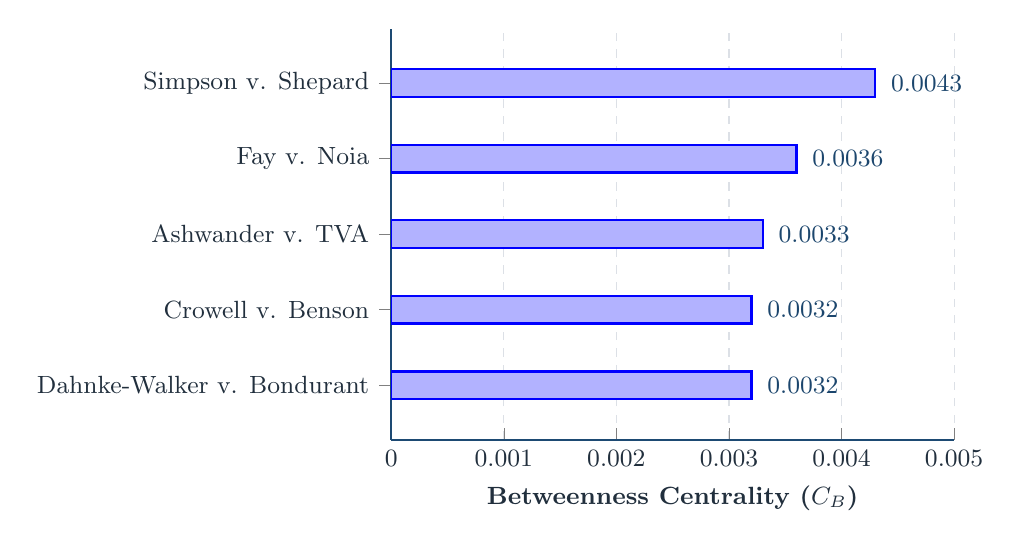
\begin{tikzpicture}
\begin{axis}[
    xbar,
    width=.72\linewidth,
    height=6.8cm,
    xmin=0,
    xmax=0.0050,
    xlabel={Betweenness Centrality ($C_B$)},
    symbolic y coords={
        {Dahnke-Walker v. Bondurant},
        {Crowell v. Benson},
        {Ashwander v. TVA},
        {Fay v. Noia},
        {Simpson v. Shepard}
    },
    ytick=data,
    y tick label style={
        font=\small,
        text=TextDark,
        anchor=east
    },
    x tick label style={
        font=\small,
        text=TextDark
    },
    xlabel style={
        font=\small\bfseries,
        text=TextDark
    },
    scaled x ticks=false,
    xtick={0,0.001,0.002,0.003,0.004,0.005},
    xticklabel style={/pgf/number format/fixed, /pgf/number format/precision=4},
    nodes near coords,
    nodes near coords style={
        font=\small\bfseries,
        text=IEEEBlue!90!black,
        anchor=west,
        xshift=2pt
    },
    nodes near coords align={horizontal},
    point meta=x,
    /pgf/number format/fixed,
    /pgf/number format/precision=4,
    bar width=10pt,
    fill=IEEEBlue!85,
    draw=IEEEBlue!95!black,
    thick,
    xmajorgrids=true,
    grid style={dashed, GridColor},
    axis lines*=left,
    enlarge y limits=0.18
]

\addplot coordinates {
    (0.0032,{Dahnke-Walker v. Bondurant})
    (0.0032,{Crowell v. Benson})
    (0.0033,{Ashwander v. TVA})
    (0.0036,{Fay v. Noia})
    (0.0043,{Simpson v. Shepard})
};

\end{axis}
\end{tikzpicture}
